\documentclass[tikz,border=2pt]{standalone}
\renewcommand{\familydefault}{\sfdefault}
\usetikzlibrary{arrows.meta,calc,positioning}
\tikzset{every picture/.style={line width=1pt, >=Stealth},
         hl/.style={fill=black, fill opacity=0.12, text opacity=1}}
\begin{document}
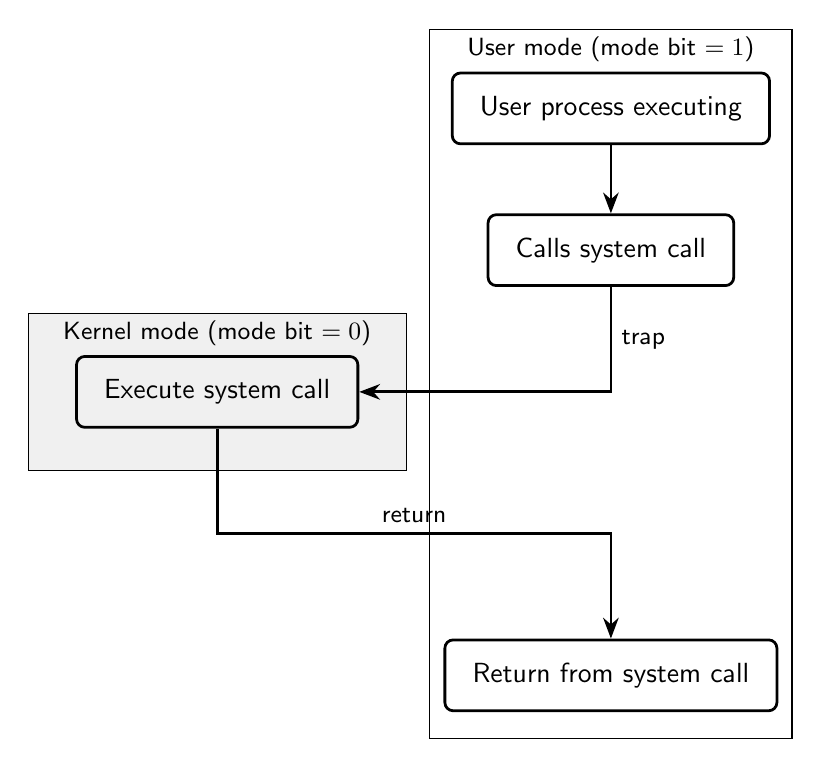
\begin{tikzpicture}[box/.style={draw, rounded corners=3pt, minimum height=0.9cm, inner xsep=10pt}]
  \node[box] (exec) at (5, 0) {User process executing};
  \node[box] (call) at (5, -1.8) {Calls system call};
  \node[box] (sys) at (0, -3.6) {Execute system call};
  \node[box] (ret) at (5, -7.2) {Return from system call};
  \draw[->] (exec) -- (call);
  \draw[->] (call) |- node[pos=0.25, right, font=\small] {trap} (sys);
  \draw[->] (sys) |- node[pos=0.75, above, font=\small] {return} (5, -5.4) -- (ret);
  % Mode regions
  \draw[thin] (2.7, 1) rectangle (7.3, -8);
  \node[font=\small] at (5, 0.75) {User mode (mode bit $= 1$)};
  \draw[thin, fill=black, fill opacity=0.06] (-2.4, -2.6) rectangle (2.4, -4.6);
  \node[font=\small] at (0, -2.85) {Kernel mode (mode bit $= 0$)};
\end{tikzpicture}
\end{document}
